\chapter{R Package singleCellFeatures}
\label{ch:singlecellfeatures}

The format in which CellProfiler feature data is stored is only of limited suitability for exploratory data analysis. CellProfiler was originally implemented in the proprietary MATLAB language but has recently been ported to Python as version 2.x, in order to move away from the drawbacks of relying on a closed-source, commercial interpreter. Unfortunately, InfectX workflows are all based on CellProfiler 1.x and there are no current plans for updating to version 2.x. Consequently, all available single cell feature data is stored as MATLAB (Level 5) MAT-files.

The way in which storage is organized, while apt for working with a limited number of features corresponding to an entire plate, is unfitting if a large number of features belonging only to a subset of cells (e.g. all cells in a specific well) are of interest. Features are saved plate-wise in individual, gzip-compressed files, typically 1--\SI{3}{\mega\byte} in size and making the data contained in several hundred (depending on pathogen and generation the analysis pipeline, 500--700 features exist) such files available to an R session\footnote{Using R version 3.2.0 \citep{RCoreTeam2015}, installed as precompiled binaries running under Mac OS 10.10.5 on a \SI{3.4}{\giga\hertz} Intel Core i7-2600 platform (iMac12,2) with \SI{32}{\giga\byte} RAM. Whenever computational timing information is given and nothing else is specified, this is the reference system used to obtain the measurements.}, using R.matlab version 3.2.0, \cite{Bengtsson2015}, takes on the order of \SI{30}{\minute}.

As MATLAB does not constitute a tool that is particularly popular in the field of statistics and does not provide many of the convenience functions, available to R, that are much appreciated in exploratory data analysis, it was decided to convert single cell feature data as generated by CellProfiler 1.x into a format natively accessible by an R environment. Due to the amount of time involved, this cannot be performed as a first step of every analysis and owing to the amount of storage necessary, it makes little sense to be carried out beforehand for all plates. Therefore, a system is needed, capable of fetching data that is not available locally, preprocessing it for direct access by R and storing the results for future use.

Furthermore, data-structures were developed, representing the hierarchy of single cell \gls{hts} data and capable of accommodating some associated metadata. Methods for operations that are frequently performed on such data are implemented in order to simplify many analysis tasks. With growing complexity of the code-base, it was decided to create an R-package that bundles the described capabilities.

Two similar projects, cellHTS2 \citep{Boutros2006} and RNAither \citep{Rieber2009}, both hosted on Bioconductor \citep{Huber2015}, were looked at but none of them fulfilled the requirements imposed by the InfectX datasets. While cellHTS2 is designed for microarray data or \gls{sirna} data obtained by a plate reader (yielding a scalar value per well), RNAither can handle data at the single cell level. It is, however, geared towards running analysis on a single feature, obtained on a single imaging channel and cannot accommodate the heterogeneity of data available from the InfectX image analysis pipeline. In addition, RNAither is neither optimized for the large amount of data associated with several hundred features, nor does it provide the sought after tools for handling such a dataset, rather than implementing a fixed analysis procedure that can be readily applied to a single intensity feature. The newly developed singleCellFeatures therefore constitutes a further step in the evolution of R packages for \gls{sirna} data analysis, starting with cellHTS2 which is generalized in a vertical fashion by RNAither with the increase in resolution from wells to cells, which in turn is extended horizontally by singleCellFeatures to include many different features.

Much effort during development of singleCellFeatures was spent for ensuring the necessary flexibility to accommodate any possible kind of feature and for implementing some crucial sections in a way that is efficient enough for interactive usage. The former task is achieved by allowing features to consist of a single value per well, a single value per cell or a vector of values per cell and only minimally relying feature naming conventions, while the latter issue is best illustrated by the following introductory example.



\begin{knitrout}
\definecolor{shadecolor}{rgb}{0.969, 0.969, 0.969}\color{fgcolor}\begin{figure}
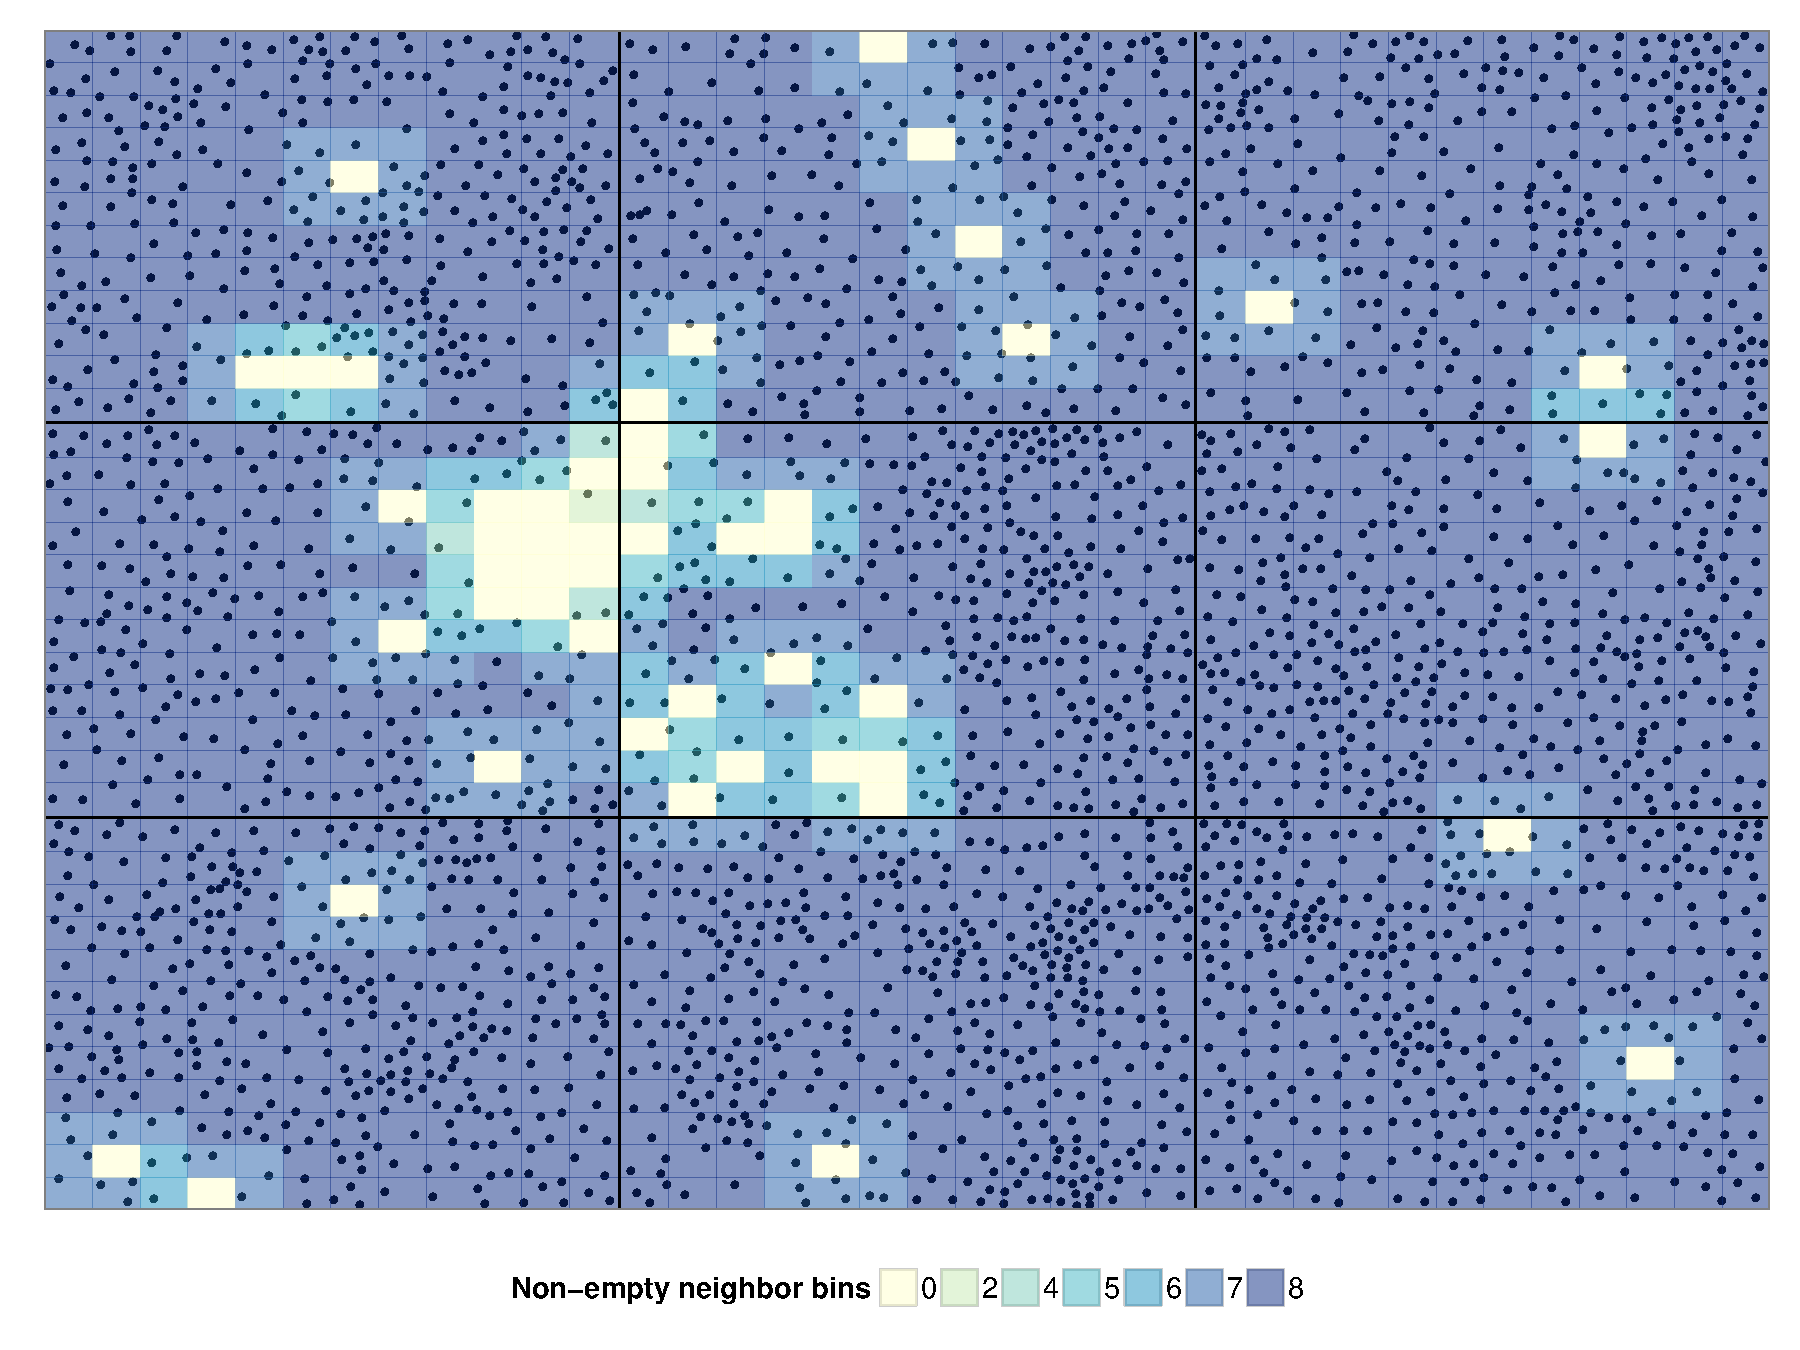
\includegraphics[width=\maxwidth]{figures/R/scf-intro/plot-scf-intro_plot-1} \caption[Visualization of cell colony edge detection by 2D binning.]{Cell colony edges are detected by 2D binning of cell center locations. Dots represent cell centers within the well H6 of plate J107-2C. Each of the nine images is segmented into 12 horizontal and 12 vertical sections yielding 144 tiles (1296 bins for the entire well). The tiles are colored according to the number of non-empty neighboring bins.}\label{fig:scf-intro_plot}
\end{figure}


\end{knitrout}


\label{ex:efficiency}
As proposed by \cite{Knapp2011} and \cite{Snijder2012}, the population context of each cell may significantly influence some morphological properties, confound phenotypic information that is measured during feature extraction and therefore has to be accounted for. They propose several features that may act as proxies to characterize aspects of population context, one of which is whether a cell is located towards the border of a colony or is surrounded by cells in all directions. In order to approximate this information from location data, an image is divided into 2-dimensional bins or facets and the number of cells per bin is counted. Cells that are located adjacent to one or more bins that are empty are considered edge cells and cells surrounded by non-empty bins are center cells. Figure \ref{fig:scf-intro_plot} visualizes the concept by color-coding facets according to the number of non-empty neighbors.

\begin{rlisting}{Calculation of population context features as implemented by \citeauthor{Knapp2011}.}{In order to detect whether a cell is located towards the border of a colony or is surrounded by neighboring cells, each well is divided into 2-dimensional bins and the number of cells per bin is counted. As implemented by \citeauthor{Knapp2011}, all bins are iterated, each of the 8 possible directions is checked for an empty neighbor and the corresponding binary value is saved to the current group of cells.}{edgepos}{p}
\begin{knitrout}\footnotesize
\definecolor{shadecolor}{rgb}{0.969, 0.969, 0.969}\color{fgcolor}\begin{kframe}
\begin{alltt}
\hlstd{edgepos} \hlkwb{<-} \hlkwa{function}\hlstd{(}\hlkwc{x}\hlstd{,} \hlkwc{y}\hlstd{,} \hlkwc{img}\hlstd{,} \hlkwc{n}\hlstd{) \{}
  \hlstd{empty} \hlkwb{<-} \hlkwd{logical}\hlstd{()}
  \hlstd{xst} \hlkwb{<-} \hlstd{img[}\hlnum{1}\hlstd{]} \hlopt{/} \hlstd{n}
  \hlstd{yst} \hlkwb{<-} \hlstd{img[}\hlnum{2}\hlstd{]} \hlopt{/} \hlstd{n}
  \hlstd{sgrid} \hlkwb{<-} \hlkwd{matrix}\hlstd{(}\hlnum{0}\hlstd{,} \hlkwc{nrow}\hlstd{=n,} \hlkwc{ncol}\hlstd{=n)}
  \hlkwa{for} \hlstd{(i} \hlkwa{in} \hlnum{1}\hlopt{:}\hlstd{n) \{}
    \hlkwa{for} \hlstd{(j} \hlkwa{in} \hlnum{1}\hlopt{:}\hlstd{n) \{}
      \hlstd{ispos} \hlkwb{<-} \hlstd{(x} \hlopt{>} \hlstd{(i} \hlopt{-} \hlnum{1}\hlstd{)} \hlopt{*} \hlstd{xst)} \hlopt{&} \hlstd{(x} \hlopt{<=} \hlstd{(i} \hlopt{*} \hlstd{xst))} \hlopt{&}
               \hlstd{(y} \hlopt{>} \hlstd{(j} \hlopt{-} \hlnum{1}\hlstd{)} \hlopt{*} \hlstd{yst)} \hlopt{&} \hlstd{(y} \hlopt{<=} \hlstd{(j} \hlopt{*} \hlstd{yst))}
      \hlstd{sgrid[i, j]} \hlkwb{<-} \hlkwd{sum}\hlstd{(ispos)}
    \hlstd{\}}
  \hlstd{\}}

  \hlkwa{for} \hlstd{(i} \hlkwa{in} \hlnum{1}\hlopt{:}\hlstd{n) \{}
    \hlkwa{for} \hlstd{(j} \hlkwa{in} \hlnum{1}\hlopt{:}\hlstd{n) \{}
      \hlstd{ispos} \hlkwb{<-} \hlstd{(x} \hlopt{>} \hlstd{(i} \hlopt{-} \hlnum{1}\hlstd{)} \hlopt{*} \hlstd{xst)} \hlopt{&} \hlstd{(x} \hlopt{<=} \hlstd{(i} \hlopt{*} \hlstd{xst))} \hlopt{&}
               \hlstd{(y} \hlopt{>} \hlstd{(j} \hlopt{-} \hlnum{1}\hlstd{)} \hlopt{*} \hlstd{yst)} \hlopt{&} \hlstd{(y} \hlopt{<=} \hlstd{(j} \hlopt{*} \hlstd{yst))}
      \hlstd{isempty} \hlkwb{<-} \hlstd{F}
      \hlkwa{if} \hlstd{((i} \hlopt{>} \hlnum{1}\hlstd{)} \hlopt{&&} \hlstd{(j} \hlopt{>} \hlnum{1}\hlstd{)} \hlopt{&&} \hlstd{(sgrid[i} \hlopt{-} \hlnum{1}\hlstd{, j} \hlopt{-} \hlnum{1}\hlstd{]} \hlopt{==} \hlnum{0}\hlstd{))}
        \hlstd{isempty} \hlkwb{<-} \hlstd{T}
      \hlkwa{else if} \hlstd{((i} \hlopt{>} \hlnum{1}\hlstd{)} \hlopt{&&} \hlstd{(sgrid[i} \hlopt{-} \hlnum{1}\hlstd{, j]} \hlopt{==} \hlnum{0}\hlstd{))}
        \hlstd{isempty} \hlkwb{<-} \hlstd{T}
      \hlkwa{else if} \hlstd{((i} \hlopt{>} \hlnum{1}\hlstd{)} \hlopt{&&} \hlstd{(j} \hlopt{<} \hlstd{n)} \hlopt{&&} \hlstd{(sgrid[i} \hlopt{-} \hlnum{1}\hlstd{, j} \hlopt{+} \hlnum{1}\hlstd{]} \hlopt{==} \hlnum{0}\hlstd{))}
        \hlstd{isempty} \hlkwb{<-} \hlstd{T}
      \hlkwa{else if} \hlstd{((j} \hlopt{>} \hlnum{1}\hlstd{)} \hlopt{&&} \hlstd{(sgrid[i, j} \hlopt{-} \hlnum{1}\hlstd{]} \hlopt{==} \hlnum{0}\hlstd{))}
        \hlstd{isempty} \hlkwb{<-} \hlstd{T}
      \hlkwa{else if} \hlstd{((j} \hlopt{<} \hlstd{n)} \hlopt{&&} \hlstd{(sgrid[i, j} \hlopt{+} \hlnum{1}\hlstd{]} \hlopt{==} \hlnum{0}\hlstd{))}
        \hlstd{isempty} \hlkwb{<-} \hlstd{T}
      \hlkwa{else if} \hlstd{((i} \hlopt{<} \hlstd{n)} \hlopt{&&} \hlstd{(j} \hlopt{>} \hlnum{1}\hlstd{)} \hlopt{&&} \hlstd{(sgrid[i} \hlopt{+} \hlnum{1}\hlstd{, j} \hlopt{-} \hlnum{1}\hlstd{]} \hlopt{==} \hlnum{0}\hlstd{))}
        \hlstd{isempty} \hlkwb{<-} \hlstd{T}
      \hlkwa{else if} \hlstd{((i} \hlopt{<} \hlstd{n)} \hlopt{&&} \hlstd{(sgrid[i} \hlopt{+} \hlnum{1}\hlstd{, j]} \hlopt{==} \hlnum{0}\hlstd{))}
        \hlstd{isempty} \hlkwb{<-} \hlstd{T}
      \hlkwa{else if} \hlstd{((i} \hlopt{<} \hlstd{n)} \hlopt{&&} \hlstd{(j} \hlopt{<} \hlstd{n)} \hlopt{&&} \hlstd{(sgrid[i} \hlopt{+} \hlnum{1}\hlstd{, j} \hlopt{+} \hlnum{1}\hlstd{]} \hlopt{==} \hlnum{0}\hlstd{))}
        \hlstd{isempty} \hlkwb{<-} \hlstd{T}
      \hlstd{empty[ispos]} \hlkwb{<-} \hlstd{isempty}
    \hlstd{\}}
  \hlstd{\}}
  \hlkwd{return}\hlstd{(empty)}
\hlstd{\}}
\end{alltt}
\end{kframe}
\end{knitrout}

\end{rlisting}

Code listing \ref{lst:edgepos} is taken from the implementation developed by \citeauthor{Knapp2011}, which was kindly supplied as supplement to their publication. While iterating over all facets, only exploiting vectorization within facets and heavily relying on if-else logic, might be a feasible approach, using datasets of the size the authors provide as exemplary material combined with permanently storing the results, such an approach is impractical with datasets as produced by InfectX. Still, the authors warn that:

\begin{quote}
These [population context feature] computations require considerable amounts of memory, and will take some time. This must be done for each of the input files, and will produce an output file containing the input data plus computed population features.
\end{quote}

\begin{rlisting}{A more efficient implementation of calculating population context features, developed for singleCellFeatures.}{Due to the larger number of cells per well and the increase in image resolution as compared to data used in \cite{Knapp2011}, calculation of border/center population context features have to be carried out in a more efficient manner, which can be accomplished by fully vectorizing the problem.}{facetBorder}{p}


\begin{rcode}
facetBorder <- function(x, y, img, facet) {
  facet.size <- img / facet
  # calculate facets (2d binning)
  x.bin <- ceiling(x / facet.size[1])
  y.bin <- ceiling(y / facet.size[2])
  # initialize empty grid/border matrices
  grid <- matrix(0, facet[2], facet[1])
  # calculate col-major grid index for each object
  index <- y.bin + (x.bin - 1) * facet[2]
  # summarize as counts
  counts <- table(index)
  # fill grid with counts
  grid[as.numeric(names(counts))] <- counts
  grid.res <- grid
  grid <- grid > 0
  # extend grid with a frame of ones
  grid.ext <- rbind(rep(1, (facet[1] + 2)),
                    cbind(rep(1, facet[2]), grid, rep(1, facet[2])),
                    rep(1, (facet[1] + 2)))
  # set up stencil
  row <- rep(rep(1:facet[2], facet[1]))
  col <- rep(1:facet[1], each=facet[2])
  colP1 <- col + 1
  colM1 <- col - 1
  rowP1 <- row + 1
  rowP2 <- row + 2
  nrowP <- facet[2] + 2
  stencil <- cbind(row   + colM1 * nrowP, # northwest neighbor
                   row   + col   * nrowP, # north neighbor
                   row   + colP1 * nrowP, # northeast neighbor
                   rowP1 + colP1 * nrowP, # west neighbor
                   rowP2 + colP1 * nrowP, # east neighbor
                   rowP2 + col   * nrowP, # southwest neighbor
                   rowP2 + colM1 * nrowP, # south neighbor
                   rowP1 + colM1 * nrowP) # southeast neighbor
  # apply stencil row-wise to grid
  border <- apply(stencil, 1, function(ind, mat) {
    return(sum(mat[ind]))
  }, as.numeric(grid.ext))
  # map col-major object index to border array
  return(border[index])
}
\end{rcode}


\end{rlisting}



\newcommand{\knitrScfRnaicellTotal}{\SI{2899.83}{\second}}
\newcommand{\knitrScfRnaicellEdgepos}{\SI{2892.67}{\second}}
\newcommand{\knitrScfRnaicellPercentage}{99.8\%}
\newcommand{\knitrScfRnaicellCellnoMean}{464}
\newcommand{\knitrScfRnaicellCellnoSd}{168}

An execution of the code, using the supplied exemplary dataset (number of cells per well: $\mu=\knitrScfRnaicellCellnoMean$, $\sigma=\knitrScfRnaicellCellnoSd$; 15 bins in x-direction and 15 bins in y-direction) reveals that of the \knitrScfRnaicellTotal\ spent on calculating population context features, \knitrScfRnaicellEdgepos\ (\knitrScfRnaicellPercentage\ of the total time) is spent on determining positions within colonies. This performance can be expected to deteriorate significantly, using InfectX data, due to a ten-fold increase in cell counts and more importantly a 3-fold rise in resolution in both x- and y direction. The surge in dataset size entails an increase in number of bins needed, to obtain sensible results (the example in figure \ref{fig:scf-intro_plot} is divided into 36 bins per dimension) and runtime scales as $\mathcal{O}(n^2)$ in number of bins per dimension.

Neither the high computational cost, and consequently not even storing the results, however are necessities, as demonstrated by a slightly optimized implementation (see listing \ref{lst:facetBorder}). Fully vectorizing the problem no longer requires the extensive use of if-else logic and due to R being an interpreted language, built for operating on vectors, such an approach can be expected to bring about compelling speed improvements. Vectorization is achieved by calculating the indices of the 8 neighboring bins for each facet and applying this stencil to the 2-dimensional matrix containing binary empty/non-empty information per bin. This efficiently yields the number of empty neighbors for each facet which then can be mapped to cells by their column-major grid indices. An additional advantage of the presented implementation is that the number of empty neighbors is obtained for free whereas the code proposed by \citeauthor{Knapp2011} would perform even worse if modified to produce this supplementary information, as the full set of if-statements has to be run to the end for each facet.



\newcommand{\knitrScfBenchmarkFacetMean}{\SI{7.77}{\milli\second}}
\newcommand{\knitrScfBenchmarkFacetSd}{\SI{2.69}{\milli\second}}
\newcommand{\knitrScfBenchmarkFacetTotal}{\SI{2.98} s}
\newcommand{\knitrScfBenchmarkEdgeMean}{\SI{515.85}{\milli\second}}
\newcommand{\knitrScfBenchmarkEdgeSd}{\SI{14.66}{\milli\second}}
\newcommand{\knitrScfBenchmarkEdgeTotal}{\SI{198.08}{\second}}
\newcommand{\knitrScfBenchmarkSpeedup}{66}

Benchmarking the two implementations reveals that a \knitrScfBenchmarkSpeedup -fold speedup is easily achievable only by completely vectorizing the problem. While the original code takes \knitrScfBenchmarkEdgeTotal\ per plate (384 iterations of the same well; $\mu=\knitrScfBenchmarkEdgeMean$, $\sigma=\knitrScfBenchmarkEdgeSd$; well H6 of plate J107-2C), total runtime is reduced to \knitrScfBenchmarkFacetTotal\ ($\mu=\knitrScfBenchmarkFacetMean$, $\sigma=\knitrScfBenchmarkFacetSd$, per well).

Such time-savings might not look that significant at first sight. But within the context of the available data, consequences of critical optimizations are of great value. First of all, interactive data analysis is sensitive to waiting times that exceed a few minutes and due to there not only being a single location feature to be analyzed, but rather 5--10, several minutes per feature are impractical. Moreover, if run-times can be sufficiently reduced, this makes it possible to run calculations on the fly instead of constantly saving results. Apart from the obvious downsides arising from storage overhead, management of result caches leads to practical issues whenever the workflow is under development and thus subject to constant change. Caches have to be invalidated and recomputed and the system overseeing these processes has to be made aware of changes, as well as understand where they apply. Furthermore, updating batches of data at once incurs substantial cost which might even be expended in vain if not all data is used before the next update triggers recomputation. Just in time generation of derived features is preferable over ahead of time calculation and the benefits justify optimization efforts.



\newcommand{\knitrScfFullPlateNSamp}{10}
\newcommand{\knitrScfFullPlateSampWell}{A1, A6, B1, B23, B9, E11, E14, I4, N20, P2}
\newcommand{\knitrScfFullPlateMyTime}{\SI{8.04}{\second}}
\newcommand{\knitrScfFullPlateRnaicellTime}{\SI{41.14}{\hour}}

When looking at runtimes of the original implementation obtained for benchmarking (\knitrScfBenchmarkEdgeTotal) and for a single execution on the supplied exemplary dataset (\knitrScfRnaicellEdgepos) side by side, a large discrepancy stands out. The two values are not directly comparable, as they are created with individual binning and differently sized datasets. But instead of explaining the divergence, these factors separate the two values even further, as the benchmarked time was obtained using a dataset roughly ten times larger and 6-fold more bins (225 versus 1296). Running the code of \citeauthor{Knapp2011} with InfectX data, as to be expected, takes significantly longer and determining cell position within colony for a single location feature over an entire plate is estimated to run for \knitrScfFullPlateRnaicellTime.\footnote{Due to the long running time, not all wells are processed, but \knitrScfFullPlateNSamp\ wells are randomly sampled and the mean per well is extrapolated to the full plate. The wells are \knitrScfFullPlateSampWell\ of plate J107-2C.} The exact same results can be computed within \knitrScfFullPlateMyTime\ by the code integrated in singleCellFeatures through vectorization as discussed previously and by splitting the data into wells.

Listing \ref{lst:edgepos} does not entirely reproduce the code of \citeauthor{Knapp2011}, but constitutes a simplified version intended for highlighting the importance of vectorization and adapted for comparison with the optimized variant. Originally, the nested for-loops iterating the bins (lines 6--12 and 14--37), are enclosed by an additional for-loop, iterating the wells. Data is stored as a large dataframe and all operations are performed on full-length vectors. The enormous number of comparisons resulting from this setup leads to serious performance issues, which are amplified when increasing the number of cells from $\sim 180000$ to $\sim 10^6$ per plate. Such observations, along with other considerations lead to development of a more sophisticated data structure for storing single cell feature data (see section \ref{sec:s3-objects}), which splits the data into smaller units and consequently eliminates constant comparisons against well indices for per-well operations.

The following sections discuss some design aspects and implementation issues of singleCellFeatures, beginning with data structures developed for representing single cell feature data, continuing with how data is acquired and locally cached, management of metadata and concluding with some tools for manipulating datasets and providing the data to third-party tools. This architectural overview is complemented by a more practical section in appendix \ref{ch:scf-manual}. For all coding, the style guide outlined in \cite{Wickham2014} was followed and \cite{Wickham2015} served as an invaluable reference, along with the extensive documentation supplied by \cite{RCoreTeam2015}. Package documentation is in-source with \mintinline{bash}{.Rd} files generated by roxygen2 \citep{Wickham2015a}.

\section{S3 Classes}
\label{sec:s3-objects}
\Gls{oop} in R can be achieved by any one of the three distinct object systems S3, S4 and \glspl{rc}. While the RC system resembles the \gls{oop} style most people coming from languages such as Java or C++ are familiar with, by implementing message-passing, features such as mutability (in-place modification of objects) and pass-by-reference semantics violate common expectations of R users. S3 and S4 objects are built on the concept of generic function \gls{oop}, which does not associate methods with classes, but employs a special type of function, called a generic function, that is responsible for method dispatch. Of the two, S3 classes are more loosely organized, lacking the formal definitions of the S4 system which can describe both representation and (multiple) inheritance. Furthermore, S4 objects are capable of multiple dispatch and all code used for creating and manipulating S4 objects is not part of base R but supplied by the methods package, which introduces a new operator, $@$, for accessing object slots.

Much base functionality in R is implemented using S3 classes, including lm and glm objects, the support for which has been available to R from its very beginning. The methods package for S4 objects is attached by default since version 1.7.0, but fewer packages make use of the newer syntax, examples include the base package stats4 and CRAN packages Matrix and lme4. Bioconductor packages on the other hand are frequently designed on top of S4 classes. \Gls{rc} was only introduced with R 2.12 as part of the methods package and therefore currently does not enjoy widespread adoption. The limitations of S3 were found to be unproblematic for the planned feature set of singleCellFeatures and due to the attractive simplicity of this scheme, several objects are implemented as S3 classes.

\subsection{Metadata Objects}


\newcommand{\knitrScfMetadatNumCol}{44}
\newcommand{\knitrScfMetadatPlateQualityStat}{\mintinline{text}{UNKNOWN}, \mintinline{text}{GOOD}, \mintinline{text}{BAD} and \mintinline{text}{WARNING}}
\newcommand{\knitrScfMetadatPlateQualityFrac}{87\%}
\newcommand{\knitrScfMetadatPlateTypes}{\mintinline{text}{ScreeningPlate}, \mintinline{text}{CheckerBoard} and \mintinline{text}{MockPlate}}
\newcommand{\knitrScfMetadatSpaces}{\mintinline{text}{INFECTX} and \mintinline{text}{INFECTX_PUBLISHED}}
\newcommand{\knitrScfMetadatGeneset}{\mintinline{text}{Drug}, \mintinline{text}{Validation}, \mintinline{text}{MicroRNAome}, \mintinline{text}{Genome} and \mintinline{text}{Kinome}}
\newcommand{\knitrScfMetadatLibrary}{\mintinline{text}{Selleck}, \mintinline{text}{Ambion}, \mintinline{text}{Sigma}, \mintinline{text}{Dharmacon} and \mintinline{text}{Qiagen}}
\newcommand{\knitrScfMetadatWellQualityStat}{\mintinline{text}{UNKNOWN}, \mintinline{text}{WARNING} and \mintinline{text}{BAD}}
\newcommand{\knitrScfMetadatWellQualityFrac}{92\%}

Metadata is extracted from aggregate files (see section \ref{sec:update-metadata}) and used to generate both plate-level and well-level metadata objects. These consist of key-value pairs stored as lists and accompany all plate-level and well-level data objects generated by singleCellFeatures. The R class attribute names are \mintinline{r}{PlateMeta data} or \mintinline{r}{WellMetadata} and both are associated with a superordinate object name \mintinline{r}{Metadata} in order to simplify method dispatch in cases where a function is able to operate on both object types. Table \ref{tab:plate-metadata} shows the 12 slots along with short descriptions that constitute a \mintinline{r}{PlateMetadata} object, while table \ref{tab:well-metadata} does the same for an object of type \mintinline{r}{WellMetadata} (20 key-value pairs in total). Several slots, namely \mintinline{r}{plate.barcode}, \mintinline{r}{plate.quality}, \mintinline{r}{experiment.name}, \mintinline{r}{experiment.pathogen}, \mintinline{r}{experiment.geneset} and \mintinline{r}{experiment.library}, are redundant and therefore only listed in table \ref{tab:plate-metadata}.

\renewcommand{\arraystretch}{1.5}
\setlength{\tabcolsep}{0.2em}
\begin{table}
  \centering
  \caption[Key-value pairs constituting the \mintinline{r}{PlateMetadata} structure.]{\mintinline{r}{PlateMetadata} structures consist of 12 key-value pairs intended to capture all relevant plate-wide metadata.}
  \label{tab:plate-metadata}
  \footnotesize
  \begin{tabular}{L{0.25\linewidth}L{0.7\linewidth}}
    Key name &
      Description \\
    \hline 
    \mintinline{r}{plate.barcode} &
      The unique identifier assigned to every plate, for example \mintinline{text}{KB02-1L}. \\
    \mintinline{r}{plate.quality} &
      Plate quality descriptors are \knitrScfMetadatPlateQualityStat, but currently most (\knitrScfMetadatPlateQualityFrac) are assigned the label \mintinline{text}{UNKNOWN}. \\
    \mintinline{r}{plate.type} &
      Possible values for plate type are \knitrScfMetadatPlateTypes\ and different types are characterized by their control layout. \\
    \mintinline{r}{experiment.space} &
      The first hierarchy level of data organization in openBIS. Current spaces are \knitrScfMetadatSpaces \\
    \mintinline{r}{experiment.group} &
      The group level is used to sort data according to pathogen (e.g. \mintinline{text}{ADENO_TEAM}). \\
    \mintinline{r}{experiment.name} &
      At the experiment level, data is grouped into screens. An example value is \mintinline{text}{ADENO-DP-K1}. \\
    \mintinline{r}{experiment.pathogen} &
      While the pathogen is already encoded in the openBIS hierarchy of InfectX, this is not necessarily so. In case of a different setup, the treatment applied to the screen can be saved separately. \\
    \mintinline{r}{experiment.geneset} &
      Different sets of genes are investigated throughout all screens and possible values are \knitrScfMetadatGeneset. \\
    \mintinline{r}{experiment.replicate} &
      Designates the replicate number of the current plate (see table \ref{tab:infectx-replicates}). \\
    \mintinline{r}{experiment.library} &
      Manufacturers that provided \gls{sirna} reagents to infectX are \knitrScfMetadatLibrary. \\
    \mintinline{r}{experiment.batch} &
      Alphanumeric identifier for the batch in which the current plate was put through the wet-lab procedure. \\
    \mintinline{r}{counts.quantiles} &
      The lower and upper 5\% quantiles for cell counts over all 3456 images of the plate, determined in order to detect bad wells. \\
    \hline 
  \end{tabular}
\end{table}

\begin{table}
  \centering
  \caption[Metadata key-value pairs that make up \mintinline{r}{WellMetadata} objects.]{Analogously to \mintinline{r}{PlateMetadata} objects, \mintinline{r}{WellMetadata} classes consist of several key-value pairs. All previously explained slots that also appear in both \mintinline{r}{Metadata} definitions are excluded from this overview (\mintinline{r}{plate.barcode}, \mintinline{r}{plate.quality}, \mintinline{r}{experiment.name}, \mintinline{r}{experiment.pathogen}, \mintinline{r}{experiment.geneset} and \mintinline{r}{experiment.library}). Please refer to table \ref{tab:plate-metadata} for more information.}
  \label{tab:well-metadata}
  \footnotesize
  \begin{tabular}{L{0.25\linewidth}L{0.7\linewidth}}
    Key name &
      Description \\
    \hline 
    \mintinline{r}{well.row} &
      Alphabetic index of the current well row (possible values are A through P). \\
    \mintinline{r}{well.col} &
      Integer-valued column index of the current well (possible values are 1--24). \\
    \mintinline{r}{well.index} &
      Well indices are calculated from row and column location and represent linearized, row-major well positions within plates. \\
    \mintinline{r}{well.type} &
      Descriptor for the type of well, the most important of which include \mintinline{text}{SIRNA}, \mintinline{text}{POOLED_SIRNA} and \mintinline{text}{CONTROL}. \\
    \mintinline{r}{well.quality} &
     Possible values for this field are \knitrScfMetadatWellQualityStat, while most wells currently are set to \mintinline{text}{UNKNOWN} (\knitrScfMetadatWellQualityFrac). \\
    \mintinline{r}{gene.name} &
      Gene symbol corresponding to the targeted gene \citep{Gray2013}. \\
    \mintinline{r}{gene.id} &
      Entrez Gene ID of the targeted gene \citep{Maglott2011}. \\
    \mintinline{r}{sirna.name} &
      The \gls{sirna} catalog ID as specified by the manufacturer. \\
    \mintinline{r}{sirna.sequence} &
      Full sequence of the 5'-3' \gls{sirna} antisense (guide) strand added to the current well. \\
    \mintinline{r}{sirna.seed} &
      The seed sequence (nucleotides 2--9 from the 5' end) of the 5'-3' \gls{sirna} guide strand. \\
    \mintinline{r}{sirna.target} &
      Sense sequence of the \gls{sirna} target. \\
    \mintinline{r}{counts.cells} &
      The cell count of the current well. \\
    \mintinline{r}{counts.pathogen} &
      Count of recognized pathogen objects (in \textit{Bartonella} screens, the number of invasomes). \\
    \mintinline{r}{counts.infection} &
      Number of infected cells according to \gls{dtis}. \\
    \hline 
  \end{tabular}
\end{table}

Having metadata structures available alongside the objects holding single cell features facilitates manipulation of the data as all relevant information is bundled and does not have to be managed separately by the user. Furthermore, information stored in \mintinline{r}{well.type} can be used for normalization (sometimes it is desirable to only normalize non-control wells) and fields like \mintinline{r}{gene.name}, \mintinline{r}{gene.id} or \mintinline{r}{sirna.name} are used often for selecting the desired subset of data. The two slots \mintinline{r}{plate.quality} and especially \mintinline{r}{well.quality} hold promise for automatically discarding bad data, but current annotation levels leave much to be desired (\knitrScfMetadatPlateQualityFrac\ and \knitrScfMetadatWellQualityFrac, respectively, are labeled as \mintinline{text}{UNKNOWN}) due to the large amount of manual labor that is involved. Perhaps, if some form of automatic quality assessment is developed or if the results from focus detection are utilized to enhance data quality comments, these fields could be put to use.

Originally, inspired by the cellHTS2 package, it was planned to use public databases for collecting further metadata, such as gene ontology, chromosomal location, gene function summaries and homology. The bioconductor package biomaRt \citep{Durinck2005,Durinck2009} can be used to query several web services, including Ensembl, Uniprot and Reactome with gene IDs \citep{Maglott2011} and retrieve gene annotations. Furthermore, \gls{sirna} sequences could be used for investigating \glspl{ote} and developing methods in order to correct for such effects. Unfortunately, time constrains so far have prevented such ideas from being explored further.

\subsection{Data Objects}
Central to the presented R package are data structures that hold single cell feature data. Instead of just storing all data as a large \mintinline{r}{data.frame} as in RNAither, a more complex scheme was developed that represents the physical hierarchy of \gls{hts} datasets. This has both the advantage of presenting an intuitive structure of the data that can easily be navigated and efficiency benefits, as selecting cells from a well does not involve $10^6$ comparisons, but selecting a slot from a list structure of length 384 (for consequences of the former approach, see the introductory example staring on page \pageref{} ).
% PlateData, WellData, ImageData

\begin{figure}
  \centering
  \begin{tikzpicture}[%
    leaf/.style={grow=down,xshift=1em,anchor=west, edge from parent path={%
      (\tikzparentnode.south) |- (\tikzchildnode.west)}
    },
    level 1/.style={sibling distance=18em},
    level 2/.style={sibling distance=4em},
    level 3/.style={sibling distance=14em},
    level 4/.style={sibling distance=4em},
    vertex style/.style={
      draw=#1,
      thick,
      fill=#1!70,
      text=white,
      minimum width=1cm,
      minimum height=0.5cm,
      font=\footnotesize
    }
  ]
    \node[vertex style=Turquoise]{PlateData}
    [edge from parent fork down]
    child{node[vertex style=SeaGreen] {PlateMetadata}
      child[leaf,level distance=6ex] {%
        node[vertex style=BurntOrange]{plate.barcode}}
      child[leaf,level distance=12ex] {%
        node[vertex style=BurntOrange]{plate.quality}}
      child[leaf,level distance=18ex] {%
        node[vertex style=BurntOrange] {plate.type}}
      child[leaf,level distance=24ex] {%
        node[vertex style=BurntOrange] {\ldots}}
      child[leaf,level distance=30ex] {%
        node[vertex style=BurntOrange] {experiment.library}}
    }
    child {node[vertex style=MidnightBlue] {data}
      child {node[vertex style=Turquoise] {A1}}
      child {node[vertex style=Turquoise] {A2}
        child {node[vertex style=SeaGreen] {WellMetadata}
          child[leaf,level distance=6ex] {%
            node[vertex style=BurntOrange]{well.index}}
          child[leaf,level distance=12ex] {%
            node[vertex style=BurntOrange]{well.type}}
          child[leaf,level distance=18ex] {%
            node[vertex style=BurntOrange] {gene.name}}
          child[leaf,level distance=24ex] {%
            node[vertex style=BurntOrange] {\ldots}}
          child[leaf,level distance=30ex] {%
            node[vertex style=BurntOrange] {sirna.sequence}}
        }
        child {node[vertex style=MidnightBlue] {data}
          child {node[vertex style=Turquoise] {img\_11}
            child[leaf,level distance=6ex] {%
              node[vertex style=BurntOrange]{image.index}}
            child[leaf,level distance=12ex] {%
              node[vertex style=BurntOrange]{\ldots}}
            child[leaf,level distance=18ex] {%
              node[vertex style=MidnightBlue]{data.vec}}
            child[leaf,level distance=24ex] {%
              node[vertex style=MidnightBlue]{data.mat}}
            child[leaf,level distance=30ex] {%
              node[vertex style=MidnightBlue] {data.lst}}
          }
          child {node[vertex style=Turquoise] {img\_12}}
          child {node[vertex style=Turquoise] {\ldots}}
          child {node[vertex style=Turquoise] {img\_33}}
        }
      }
      child {node[vertex style=Turquoise] {\ldots}}
      child {node[vertex style=Turquoise] {P24}}
    };
  \end{tikzpicture}
  \caption[Data structure used for representing a complete plate of single cell data.]{Single cell data is organized according to the hierarchy imposed by \gls{hts} experiment design. Plates are divided into wells which are subdivided into images and Metadata objects (green) are attached at each level. Data objects provided by singleCellFeatures are in light blue and contain lists of subordinate objects (dark blue), while Metadata objects consist of key-value pairs (orange).}
  \label{fig:scf-platedata}
\end{figure}

\subsection{Auxiliary Objects}
%PlateAggregate, MatData, PlateLocation, WellLocation

\section{Data Import}
\label{sec:data-import}
% include integrity check
\section{Metadata Management}
\label{sec:metadata-management}

\section{Data Manipulation}
% add, remove, melt
